% Created 2023-10-29 Sun 16:15
% Intended LaTeX compiler: pdflatex
\documentclass{article}
\usepackage[utf8]{inputenc}
\usepackage[T1]{fontenc}
\usepackage{graphicx}
\usepackage{longtable}
\usepackage{wrapfig}
\usepackage{rotating}
\usepackage[normalem]{ulem}
\usepackage{amsmath}
\usepackage{amssymb}
\usepackage{capt-of}
\usepackage{hyperref}
\usepackage{minted}

        \hypersetup{ colorlinks,% 
                linkcolor=blue,% 
                citecolor=black,%
                urlcolor=black,%
                filecolor=black
               }

        \usepackage{array}
        \usepackage{xcolor}
        \definecolor{bg}{rgb}{0.95,0.95,0.95}

\usepackage[innermargin=1.5in,outermargin=1.25in,vmargin=3cm]{geometry}
\linespread{1.3}
\author{Oscar Qi}
\date{\today}
\title{}
\hypersetup{
 pdfauthor={Oscar Qi},
 pdftitle={},
 pdfkeywords={},
 pdfsubject={},
 pdfcreator={Emacs 29.1 (Org mode 9.6.6)}, 
 pdflang={English}}
\begin{document}

\tableofcontents


\section{Something need to install}
\label{sec:org899eb59}
\begin{minted}[bgcolor=bg,frame=lines,linenos=,fontsize=\scriptsize]{shell}
sudo apt install texlive-xelatex gnuplot plantuml
pip install pygmentize-faster
\end{minted}

\section{Writing on Emacs}
\label{sec:org98f6ab2}

\url{https://github.com/thinkhuman/writingwithemacs}



\section{test Only}
\label{sec:orge40959c}
\begin{table}[htbp]
\caption{my image}
\centering
\begin{tabular}{p{0.3\textwidth}|p{0.3\textwidth}}
title & title\\[0pt]
\hline
\begin{center}
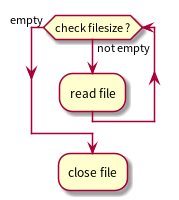
\includegraphics[width=.9\linewidth]{./imgs/test.png}
\end{center} & \begin{center}
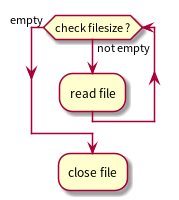
\includegraphics[width=.9\linewidth]{./imgs/test.png}
\end{center}\\[0pt]
\end{tabular}
\end{table}

\begin{center}
\begin{tabular}{rrrrr}
1 & 2 & 3 & 4 & 5\\[0pt]
\hline
\hline
1 & 2 & 2 & 33 & 4\\[0pt]
\hline
\end{tabular}
\end{center}



\begin{center}
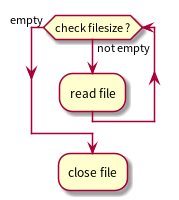
\includegraphics[height=0.5\textwidth]{./imgs/test.png}
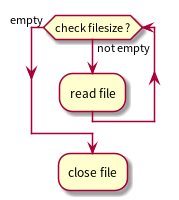
\includegraphics[height=0.5\textwidth]{./imgs/test.png}
\end{center}


\begin{wrapfigure}{r}{0.4\textwidth}
\centering
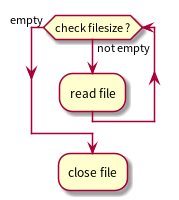
\includegraphics[width=0.38\textwidth]{./imgs/test.png}
\caption{\label{fig:org256f208}An image}
\end{wrapfigure}





\begin{minted}[bgcolor=bg,frame=lines,linenos=,fontsize=\scriptsize]{sh}
ls -la
\end{minted}

\begin{minted}[bgcolor=bg,frame=lines,linenos=,fontsize=\scriptsize]{java}
int main(int argc, char *argv[])
{
        printf("test....\n");

        return 0;
}
\end{minted}



\begin{table}[htbp]
\label{tab:orge708a14}
\centering
\begin{tabular}{lrr}
Ben & 9.2 & 9.9\\[0pt]
Tim & 6.7 & 7.7\\[0pt]
Tom & 7.5 & 6.7\\[0pt]
Dean & 8.0 & 7.0\\[0pt]
\end{tabular}
\end{table}

\begin{minted}[bgcolor=bg,frame=lines,linenos=,fontsize=\scriptsize]{gnuplot}
set title "Students' Grades"
set yrange[0:10]
set style data histogram
set terminal png size 400,300

set macros
png="set terminal png size 1800,1800 crop enhanced font \"/usr/share/fonts/truetype/times.ttf,30\" dashlength 2; set termoption linewidth 3"
eps="set terminal postscript fontfile \"/usr/share/fonts/truetype/times.ttf\"; set termoption linewidth 3;

set style line 1 linecolor rgb '#de181f' linetype 1  # Red
set style line 2 linecolor rgb '#0060ae' linetype 1  # Blue
set style line 3 linecolor rgb '#228C22' linetype 1  # Forest green

set style line 4 linecolor rgb '#18ded7' linetype 1  # opposite Red
set style line 5 linecolor rgb '#ae4e00' linetype 1  # opposite Blue
set style line 6 linecolor rgb '#8c228c' linetype 1  # opposite Forest green
plot x ls 1, -x ls 2, x**3 ls 3

plot data using 2:xtic(1) title 'Maths', '' using ($3) title 'Physics'
\end{minted}


\section{Maybe usefull}
\label{sec:orgd8ee9c4}
\url{https://github.com/linktohack/ox-latex-subfigure}
\end{document}